\documentclass[12pt]{article}

\usepackage{times}
\usepackage{geometry}
\geometry{margin=1in}
\usepackage{graphicx}
\usepackage{amsmath}
\usepackage{booktabs}
\usepackage{array}
\usepackage{setspace}

\newcounter{algorithm}
\newenvironment{algorithmbox}[2]{%
    \refstepcounter{algorithm}%
    \begin{center}
    \begin{minipage}{0.92\textwidth}
    \singlespacing
    \small
    \hrule
    \vspace{0.4em}
    \noindent\textbf{Algorithm \thealgorithm: #2}\label{#1}
    \vspace{0.4em}
    \hrule
    \vspace{0.5em}
    \renewcommand{\arraystretch}{1.18}
    \begin{tabular}{@{}r p{0.80\textwidth}@{}}
}{%
    \end{tabular}
    \vspace{0.4em}
    \hrule
    \end{minipage}
    \end{center}
}
\newcommand{\algmeta}[2]{\multicolumn{2}{@{}p{0.88\textwidth}@{}}{\textbf{#1:} #2}\\[0.15em]}
\newcommand{\algstep}[2]{#1 & #2\\}

\title{Beam Search for Neuro-Symbolic Equation Recognition}
\author{Evan Hammam}
\date{March 2026}

\begin{document}

\doublespacing

\maketitle

\begin{abstract}
This paper evaluates beam search as a decoder for equation recognition that combines neural probabilities with symbolic constraints. A convolutional neural network supplies probabilities for each symbol, and a separate decoder then selects a complete expression whose symbols have high CNN probabilities and whose arithmetic is valid. This requires joint inference over all five symbol positions rather than isolated greedy classification. The benchmark consists of single-digit equations of the form $d_1 \text{ } op \text{ } d_2 = d_3$. The domain is kept deliberately small so that exhaustive decoding remains tractable. Exhaustive decoding scores every valid equation and serves as an exact reference for measuring approximate methods. Since exhaustive decoding does not scale well to larger symbolic domains, this investigation asks how much accuracy is lost if beam search is used as an alternative. To test robustness across different levels of perceptual difficulty, Gaussian noise is applied to the input images at increasing intensities. This degrades CNN confidence and forces the decoder to choose among competing valid equations. On a held-out set of 5{,}000 fixed-seed equations, wider beams progressively approach the exhaustive reference. Under noise $\sigma=0.4$, a beam width of $K=10$ reaches 92.38\% equation accuracy and retains the correct equation in the final beam for 96.18\% of examples. A beam width of $K=50$ reaches 93.80\% and matches exhaustive decoding. Beam search is effective when the correct equation is not pruned too early. Under heavy noise, however, the CNN may assign a higher probability to a different equation that is also arithmetically valid.

\end{abstract}

\section{Introduction}
Many prediction tasks require individual predictions to satisfy a shared global constraint, a setting commonly treated as structured prediction~\cite{bakir2007,lafferty2001,tsochantaridis2005}. A neural model may assign high probability to individual fields, symbols, or objects, but the final output must be coherent as a whole. Systems must select labels that operate together rather than simply choose the highest-probability label at each position. This challenge is relevant to tasks where local predictions must combine into one valid structure, such as parsing a sentence, extracting fields from a document, generating syntactically valid code, identifying objects in a spatially consistent scene, or recognizing symbols that form a valid mathematical expression~\cite{collins2004,peng2006,gulwani2017,mao2019,zanibbi2012}.

The central question is how to decode a constrained output from uncertain neural predictions. This paper examines the use of beam search as a decoder. Beam search is an approximate structured-inference procedure that builds an output incrementally, retains the top-$K$ partial hypotheses at each step, and discards the remainder~\cite{collins2004,sutskever2014,bahdanau2015}. Its cost depends on the beam width rather than on the number of possible complete outputs. Beam search is useful here because it exposes whether the correct partial output is discarded early and no subsequent symbolic check can recover it. This is an important failure mode to examine.

Predicting the values of digits under arithmetic constraints is used as a controlled benchmark task to investigate this challenge. Each input image contains an expression of the form $d_1 \; op \; d_2 = d_3$. A convolutional neural network assigns a probability distribution over 13 symbol classes for each of the five positions, and the decoder then searches over partial equations and applies arithmetic validity at the final step. The CNN supplies local estimates of the digit values, and the decoder selects the complete equation.

The distinction between validity and correctness is relevant here. When the image displays $3+2=5$, the prediction $4+1=5$ remains arithmetically valid even though it fails to match the image. The constraint eliminates invalid equations without guaranteeing the correct one, so whenever the CNN assigns a higher score to a valid equation that differs from the true equation, the decoder may still select it.

The benchmark has been kept deliberately small, with only 110 arithmetically valid equations, which enables beam search to be compared directly against exhaustive decoding. This allows errors to be separated between search mistakes, where beam search removes the correct equation too early, and ranking mistakes, where the CNN assigns a higher probability to a different valid equation. The main contribution is a reproducible analysis of how beam width affects accuracy, oracle accuracy, pruning, rank, and symbolic search cost.

\section{Related Work}
Prior work on probabilistic logic and neuro-symbolic reasoning supports this separation between the neural recognition step and the symbolic reasoning step. DeepProbLog incorporates neural predicates into probabilistic logic programs~\cite{manhaeve2018}, and ProbLog assigns probabilities to uncertain facts and logical proofs~\cite{deraedt2007}. This implementation does not use a probabilistic logic program, a proof graph, or train the neural model with logic-aware objectives, but it borrows the idea that reasoning steps may be used to choose among constrained outputs from probabilistic neural predictions. Other neuro-symbolic systems separate perception from reasoning as well. Mao et al.\ connect visual perception to symbolic reasoning over concepts and relations~\cite{mao2019}, and Dong et al.\ examine neural architectures for logical and relational reasoning~\cite{dong2019}. The same design principle applies here. The CNN provides uncertain local evidence, and the decoder evaluates candidate interpretations using structure that independent symbol classification cannot represent.

Beam search is commonly used in settings where exact search is impractical. Neural machine translation systems use beam decoding to maintain several high-probability partial translations~\cite{sutskever2014,bahdanau2015}, and incremental parsers use beam search to explore partial syntactic analyses~\cite{collins2004}. The decoder developed in this paper applies the same algorithmic pattern to constrained equation recognition.

Several alternative structured-prediction frameworks could in principle combine local evidence with global constraints. Conditional random fields combine local information with structured output constraints using undirected probabilistic graphs~\cite{lafferty2001}. A linear-chain CRF would be suitable if the global structure depended on adjacency, such as whether a digit is likely to follow an operator. In this case, however, the symbols $d_1$, $op$, $d_2$, and $d_3$ interact through a non-local arithmetic relationship~\cite{kschischang2001}. An integer-programming or constraint-programming decoder could be used to optimize the same log-probability objective under the arithmetic constraint~\cite{roth2004}, and structured support vector machines and related large-margin methods could also be used to select the highest-scoring candidate satisfying task constraints~\cite{tsochantaridis2005}.

The relevance of these approaches depends on the particular modeling assumptions of the task. A CRF or structured SVM is well suited in cases where the relevant structure should be learned from data. A factor graph or constraint solver is relevant when the constraints have a clear graph or optimization form. Probabilistic logic is appropriate when the rules are relational or themselves uncertain. However, the beam search decoder depends only on candidate expansions, neural scores, and a validity function.

\section{Methodology}
The system has three stages. The input expression image is first split into five fixed symbol crops. A CNN then assigns a probability distribution for each symbol, and a beam decoder maintains a bounded set of partial hypotheses while searching for a high-scoring assignment that satisfies the arithmetic constraint. To keep the scope narrow, the system assumes a fixed five-symbol layout of basic addition or subtraction arithmetic and performs no segmentation or multi-digit arithmetic. The goal is to determine whether a known symbolic constraint can improve final predictions when the neural prediction is uncertain.

Gaussian noise is used as a controlled image corruption to vary the difficulty of the perceptual input~\cite{hendrycks2019}. Images are first represented with pixel values in $[0,1]$. For each noise condition, independent noise $\epsilon \sim \mathcal{N}(0,\sigma^2)$ is added to every pixel before CNN classification, and the resulting image is clipped back to $[0,1]$. The case $\sigma=0.0$ uses the original image without perturbation.

\section{Dataset}
The training set consists of 60{,}000 MNIST digits and 300 rendered operator images of ``+'', ``-'', and ``=''~\cite{lecun1998}. Together, these images define 13 symbols, including ten digits and three operators. The held-out set of expressions contains 5{,}000 equations composed of MNIST test digits, each of the form $d_1 \; op \; d_2 = d_3$ and represented as a $28 \times 140$ image obtained by concatenating five $28 \times 28$ cropped images. Addition examples use operands $a,b \in \{0,\dots,4\}$, while subtraction examples use $a \in \{5,\dots,9\}$ and $b \in \{0,\dots,4\}$. Figure~\ref{fig:qualitative} shows example expressions in the held-out equation set.

\begin{figure}[t]
    \centering
    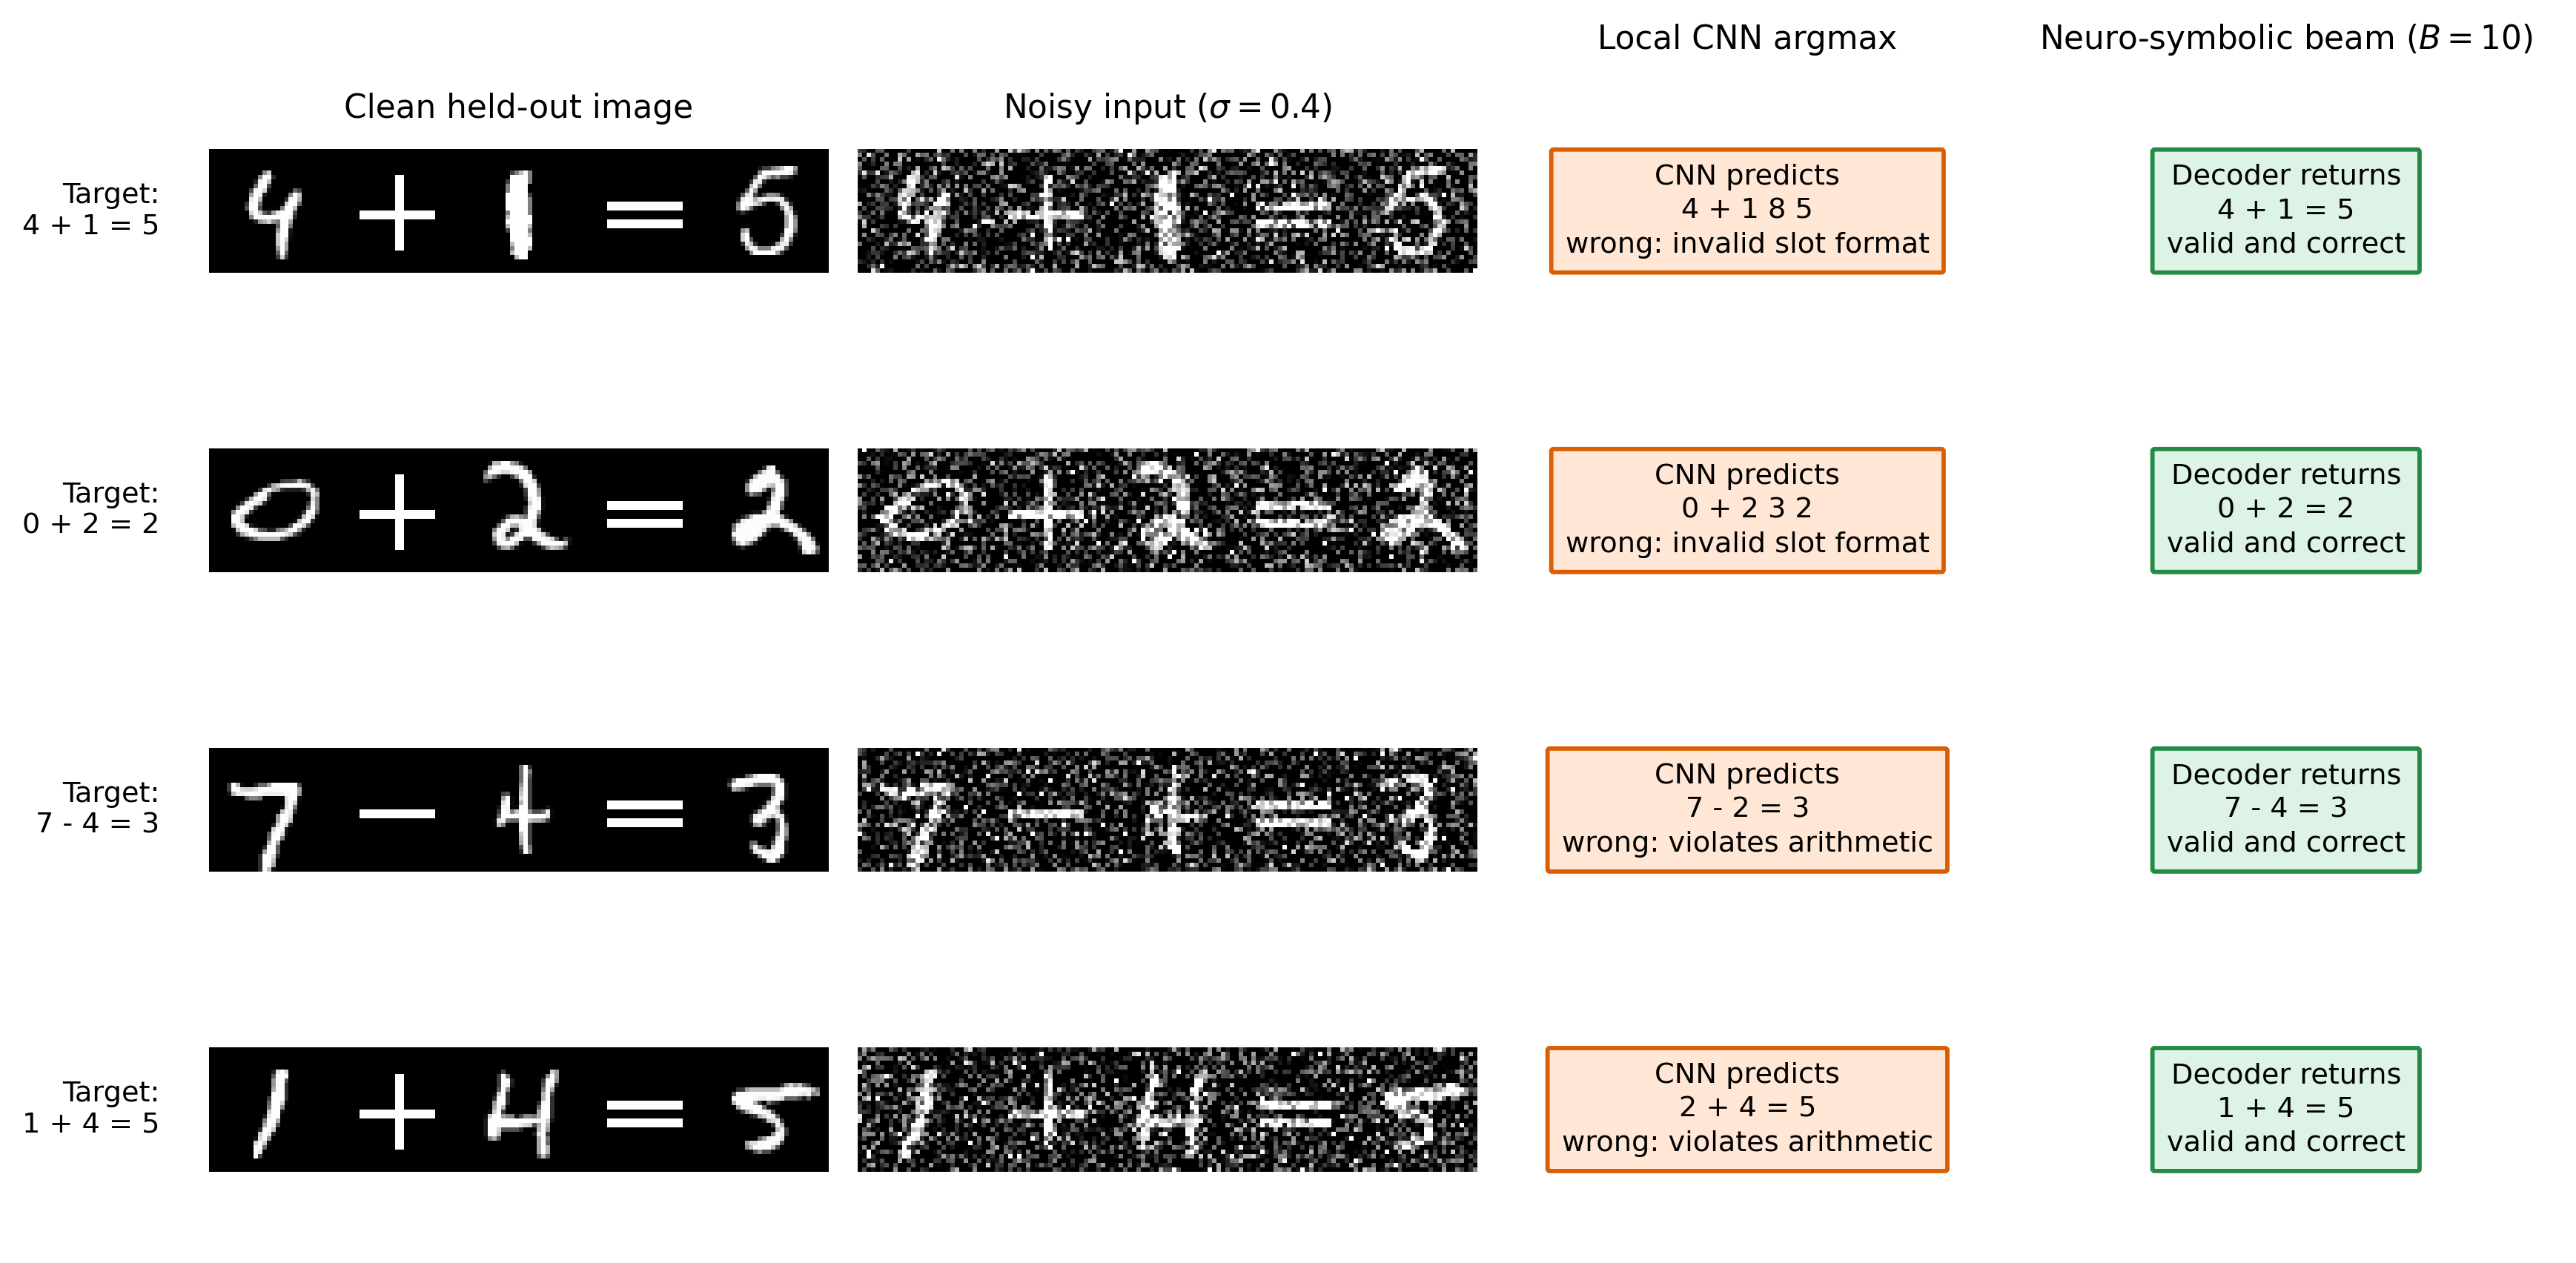
\includegraphics[width=\textwidth]{qualitative_decoding_examples.png}
    \caption{Qualitative examples drawn from the held-out equation set.}
    \label{fig:qualitative}
\end{figure}

\section{Model}
The perception module is a compact CNN consisting of two $3 \times 3$ convolutional layers with ReLU activations, $2 \times 2$ max pooling, a 128-unit hidden layer, and a 13-class output layer, for a total of 422{,}029 trainable parameters. The model is trained with cross-entropy loss and the Adam optimizer at learning rate 0.001 for five epochs~\cite{kingma2015}. The final experiments load the saved checkpoint rather than retraining the entire network. At inference time, each expression image is divided into five crops, and for position $i$ the CNN outputs a probability distribution
\[
p_i(y_i), \qquad i \in \{1,\dots,5\},
\]
where $y_i$ ranges over the 13 symbol classes. These probability distributions are the sole input to the symbolic decoder. Because candidate equations are scored by the product of their per-symbol probabilities, the constraint can correct a wrong top-scoring prediction only when the correct symbol retains nonzero probability at every position.

\section{Symbolic Decoder}
The symbolic decoder enforces the validity of the arithmetic structure without requiring the valid set to be enumerated in advance of the search. The unconstrained classifier can assign 13 possible symbols at each of the five positions, yielding $13^5 = 371{,}293$ possible symbol sequences. The fixed layout restricts positions 1, 3, and 5 to digits, position 2 to $+$ or $-$, and position 4 to $=$, leaving $10 \times 2 \times 10 \times 1 \times 10 = 2{,}000$ syntactically valid assignments, of which only 110 also satisfy the arithmetic constraint. The relatively small space of valid configurations enables an exhaustive decoder to be benchmarked. Beam search nevertheless remains the primary decoder of interest, since the goal is to evaluate how approximate search behaves relative to that reference.

Figure~\ref{fig:searchspace} shows this reduction step by step. The blue bars indicate the number of candidates expanded or evaluated at each position, and the green bars indicate the number retained after pruning or validity filtering. In the exhaustive panel, the decoder ultimately scores the 110 arithmetically valid equations. In the beam-search panels, the decoder keeps at most $B$ partial equations after each position, so the retained set can be much smaller than the full search tree.

\begin{figure}[t]
    \centering
    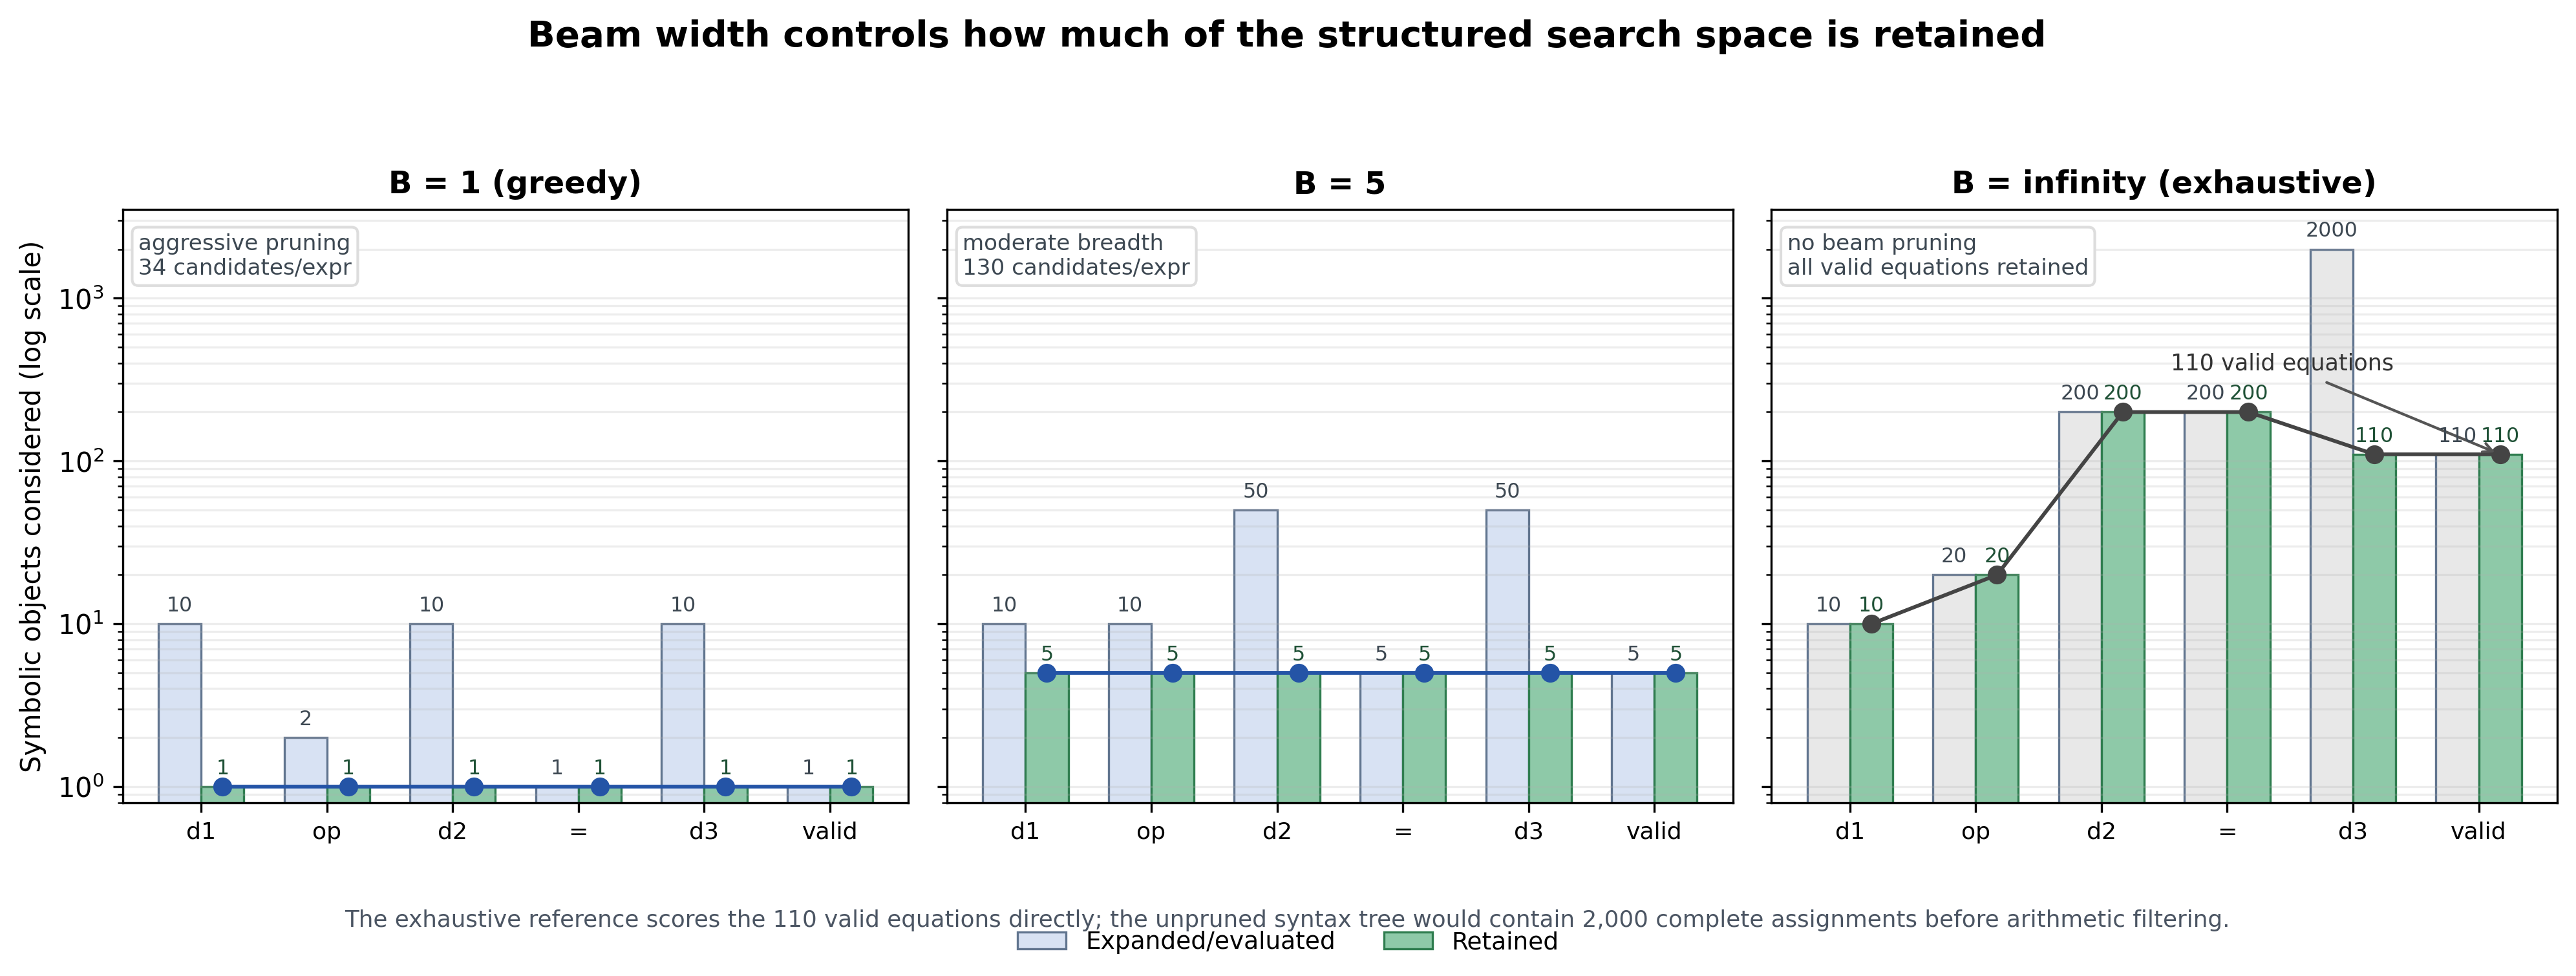
\includegraphics[width=\textwidth]{search_space_reduction.png}
    \caption{Search-space reduction during decoding. }
    \label{fig:searchspace}
\end{figure}

An unconstrained local predictor chooses each position independently according to
\[
\tilde{y}_i = \arg\max_k p_i(k),
\]
whereas an exhaustive neuro-symbolic decoder instead solves a constrained maximum a posteriori (MAP) problem. Here, MAP means choosing the valid equation with the highest product of CNN symbol probabilities. The decoder computes
\begin{equation}
\hat{\mathbf{y}} = \arg\max_{\mathbf{y} \in \mathcal{V}} \prod_{i=1}^{5} p_i(y_i).
\label{eq:map}
\end{equation}
Exhaustive decoding sums log probabilities and selects the highest-scoring valid equation. This decoder can be interpreted as Bayesian conditioning on symbolic validity. The neural model defines a factorized distribution
\[
p_{\text{NN}}(\mathbf{y}) = \prod_{i=1}^{5} p_i(y_i),
\]
and the symbolic decoder restricts that distribution to the valid set,
\[
p_{\text{NS}}(\mathbf{y}) =
\frac{p_{\text{NN}}(\mathbf{y}) \mathbf{1}[\mathbf{y} \in \mathcal{V}]}
{\sum_{\mathbf{y}' \in \mathcal{V}} p_{\text{NN}}(\mathbf{y}')}.
\]
In other words, the symbolic decoder removes invalid equations and redistributes the probability mass over what remains. Exhaustive decoding computes this distribution exactly, making it the reference against which approximate procedures can be measured.

\subsection{Beam Search Decoder}
Beam search approximates constrained MAP by maintaining a limited set of partial assignments. Exhaustive decoding scores every valid complete equation and selects the one with the highest CNN score, while beam search constructs equations one symbol at a time and retains only the top $B$ partial candidates after each step. At every position, the decoder adds the relevant log probability to each extension, prunes to the $B$ highest-scoring partial assignments, and applies the arithmetic constraint to filter completed assignments. The candidate-label function $C(i)$ specifies the labels permitted at position $i$, returning $\{0,\dots,9\}$ at digit positions, $\{+,-\}$ at the operator position, and $\{=\}$ at the equality position.

The search procedure is given in Algorithm~\ref{alg:beam-search} of Appendix~\ref{app:algorithms}, and the equation-specific validity check appears as Algorithm~\ref{alg:valid-equation}. Adapting the decoder to a different constrained-prediction task would require modifying the candidate labels and validity function, while the beam-search procedure itself would remain unchanged. The beam width controls the tradeoff between search cost and candidate retention. A narrow beam risks pruning the correct prefix before the arithmetic constraint is applied, while a wider beam preserves a larger set of alternatives at greater computational cost. Beam search does not require a precomputed set of valid outputs, which is essential for tractability in larger domains.

\section{Experimental Protocol}
The final evaluation compares constrained beam search against an exhaustive reference decoder that evaluates all 110 valid equations. Beam search is tested with $B \in \{1,3,5,10,20,50,110\}$, alongside an exhaustive row denoted $B=\infty$. The use of multiple beam widths exposes beam search's behavior as the beam grows and makes the underlying error sources easier to identify. A pruning failure arises when the correct partial equation is removed from the beam before decoding completes. A ranking failure occurs when the correct equation is still in the beam, but another valid equation has a higher CNN score. A third failure can occur when the neural probabilities supply too little support to the true symbols for the correct equation to remain competitive at all.

The reported metrics are symbol accuracy, equation accuracy, oracle accuracy, the rank of the correct equation when present, and search cost. Oracle accuracy measures whether the beam retained the correct answer at any rank, while actual equation accuracy measures whether the decoder ranked that answer first. The gap between the two quantifies cases in which search succeeded in retaining the answer but scoring selected a different valid equation. Gaussian image noise with $\sigma \in \{0.0, 0.2, 0.4, 0.6\}$ is applied prior to classification, and the evaluation records prefix survival, final-beam membership, and correct-equation rank at each beam width.

\section{Results}
Table~\ref{tab:results} reports equation accuracy across beam widths and noise levels. Accuracy converges toward the exhaustive reference as the beam widens, with clean and mildly noisy inputs plateauing by $B=5$ and $B=10$. At $\sigma=0.4$, the exhaustive value is recovered by $B=50$, while at $\sigma=0.6$ it is recovered by $B=110$. Under $\sigma=0.4$, widening the beam from $B=1$ to $B=10$ raises equation accuracy from 59.96\% to 92.38\%, and a further increase to $B=50$ produces 93.80\% accuracy, equal to that of exhaustive decoding. The decoder therefore does not need to retain every valid equation in order to recover most of the exhaustive accuracy, although it must preserve the true prefix long enough for arithmetic validity to influence the final decision.

\begin{table}[t]
    \centering
    \caption{Main beam-search results, reporting equation accuracy (\%) as a function of beam width.}
    \label{tab:results}
    \small
    \begin{tabular}{lrrrrrrrr}
        \toprule
        Noise & $B=1$ & $B=3$ & $B=5$ & $B=10$ & $B=20$ & $B=50$ & $B=110$ & $B=\infty$ \\
        \midrule
        $\sigma=0.0$ & 97.24 & 99.86 & 100.00 & 100.00 & 100.00 & 100.00 & 100.00 & 100.00 \\
        $\sigma=0.2$ & 96.32 & 99.76 & 99.94 & 100.00 & 100.00 & 100.00 & 100.00 & 100.00 \\
        $\sigma=0.4$ & 59.96 & 82.62 & 88.14 & 92.38 & 93.66 & 93.80 & 93.80 & 93.80 \\
        $\sigma=0.6$ & 6.24 & 16.94 & 23.56 & 32.02 & 38.12 & 41.66 & 41.98 & 41.98 \\
        \bottomrule
    \end{tabular}
\end{table}

\begin{figure}[t]
    \centering
    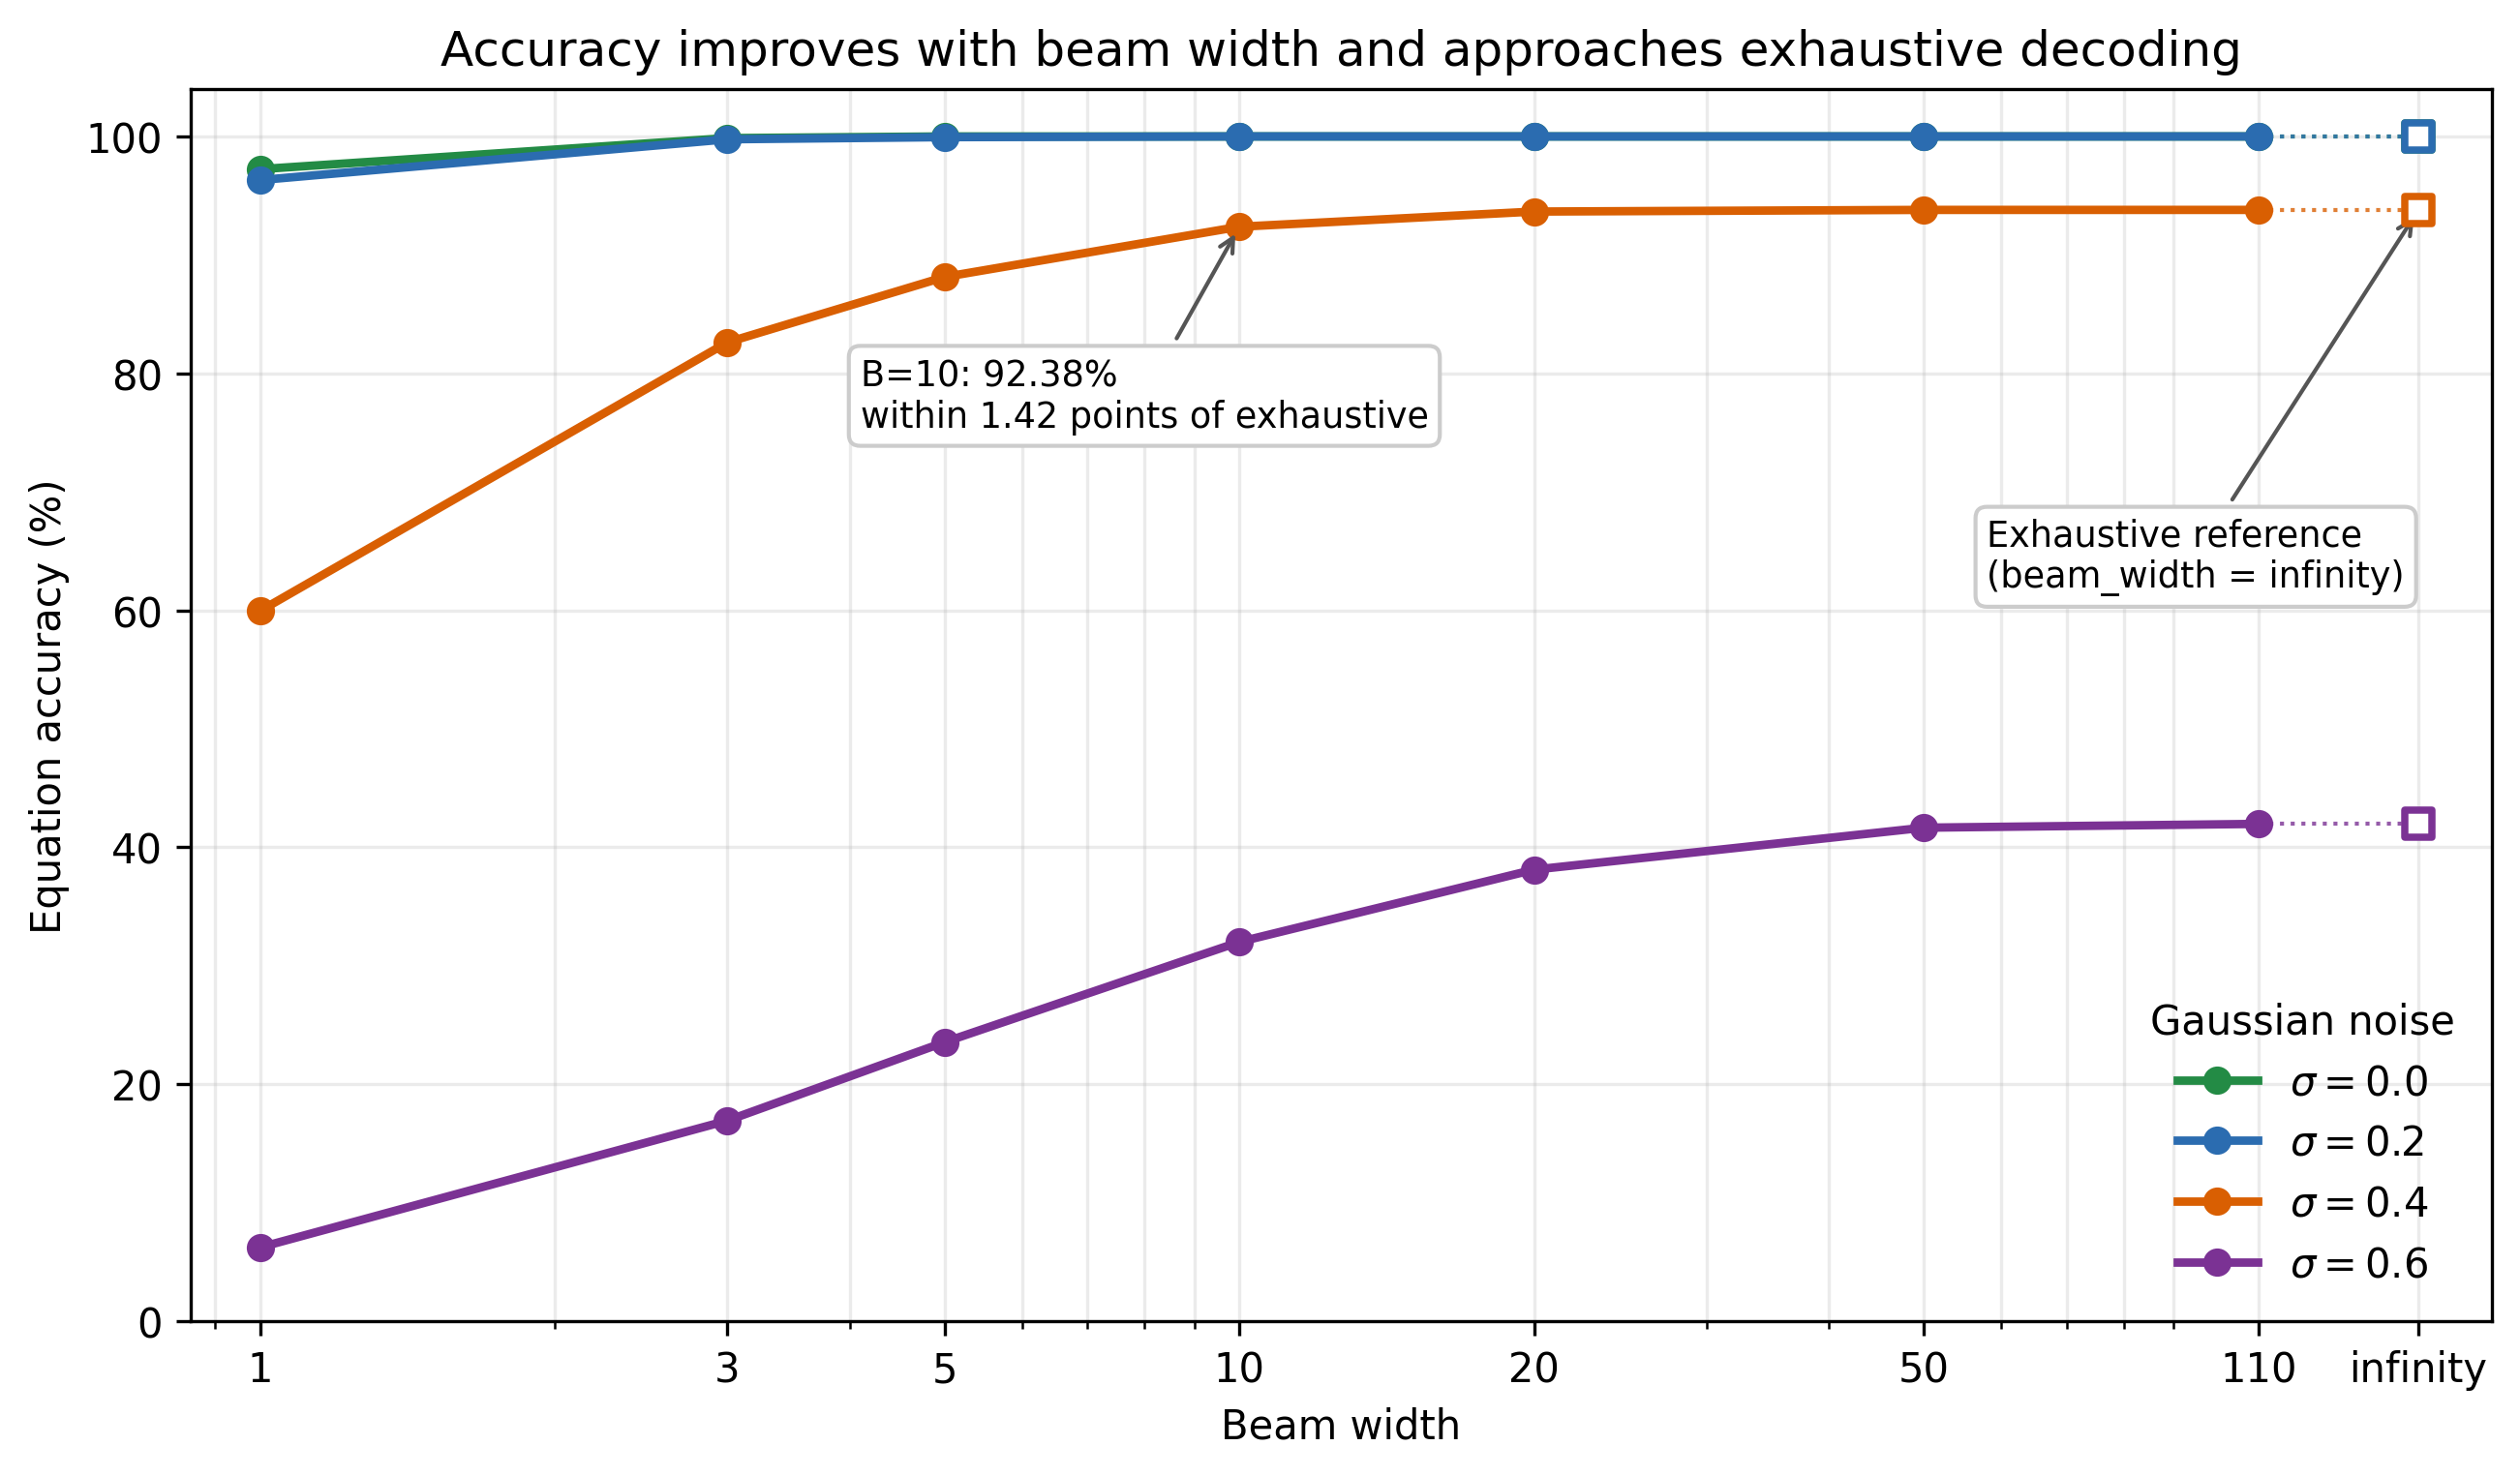
\includegraphics[width=0.9\textwidth]{beam_width_accuracy.png}
    \caption{Equation accuracy as a function of beam width under Gaussian image noise.}
    \label{fig:beamwidth}
\end{figure}

Table~\ref{tab:efficiency} reports the symbolic search cost. These timings reflect only the symbolic search step and exclude CNN probability extraction. Exhaustive decoding performs well because it scores only the 110 known valid equations within a simple loop. Beam width $B=10$ is slower than exhaustive decoding in wall-clock time, although it requires fewer log-probability additions overall, performing 240 score computations per expression compared with 550 for exhaustive decoding.

The search-error analysis examines whether the true equation appears in the final valid beam even when it fails to be ranked first. Table~\ref{tab:recoverability} reports this analysis at $\sigma=0.4$. At $B=10$, the correct equation is present in the final beam for 96.18\% of examples, has mean rank 1.04 when present, and is pruned before the final beam for the remaining 3.82\% of examples. The corresponding equation accuracy of 92.38\% is lower because a portion of the correct equations that survive in the beam are still ranked below an alternative valid equation.

\begin{table}[t]
    \centering
    \caption{Search efficiency for symbolic decoding only.}
    \label{tab:efficiency}
    \small
    \begin{tabular}{lrrrr}
        \toprule
        Decoder & Candidates/expr & Score ops/expr & Time/expr (ms) & Wall-clock speedup \\
        \midrule
        $B=1$ & 34.0 & 33.0 & 0.0318 & 2.458 \\
        $B=3$ & 82.0 & 79.0 & 0.0543 & 1.439 \\
        $B=5$ & 130.0 & 125.0 & 0.0783 & 0.998 \\
        $B=10$ & 250.0 & 240.0 & 0.1404 & 0.556 \\
        $B=20$ & 470.0 & 450.0 & 0.2524 & 0.309 \\
        $B=50$ & 830.0 & 780.0 & 0.7150 & 0.109 \\
        $B=110$ & 1550.0 & 1440.0 & 1.3633 & 0.057 \\
        Exhaustive & 110.0 & 550.0 & 0.0781 & 1.000 \\
        \bottomrule
    \end{tabular}
\end{table}

\begin{figure}[t]
    \centering
    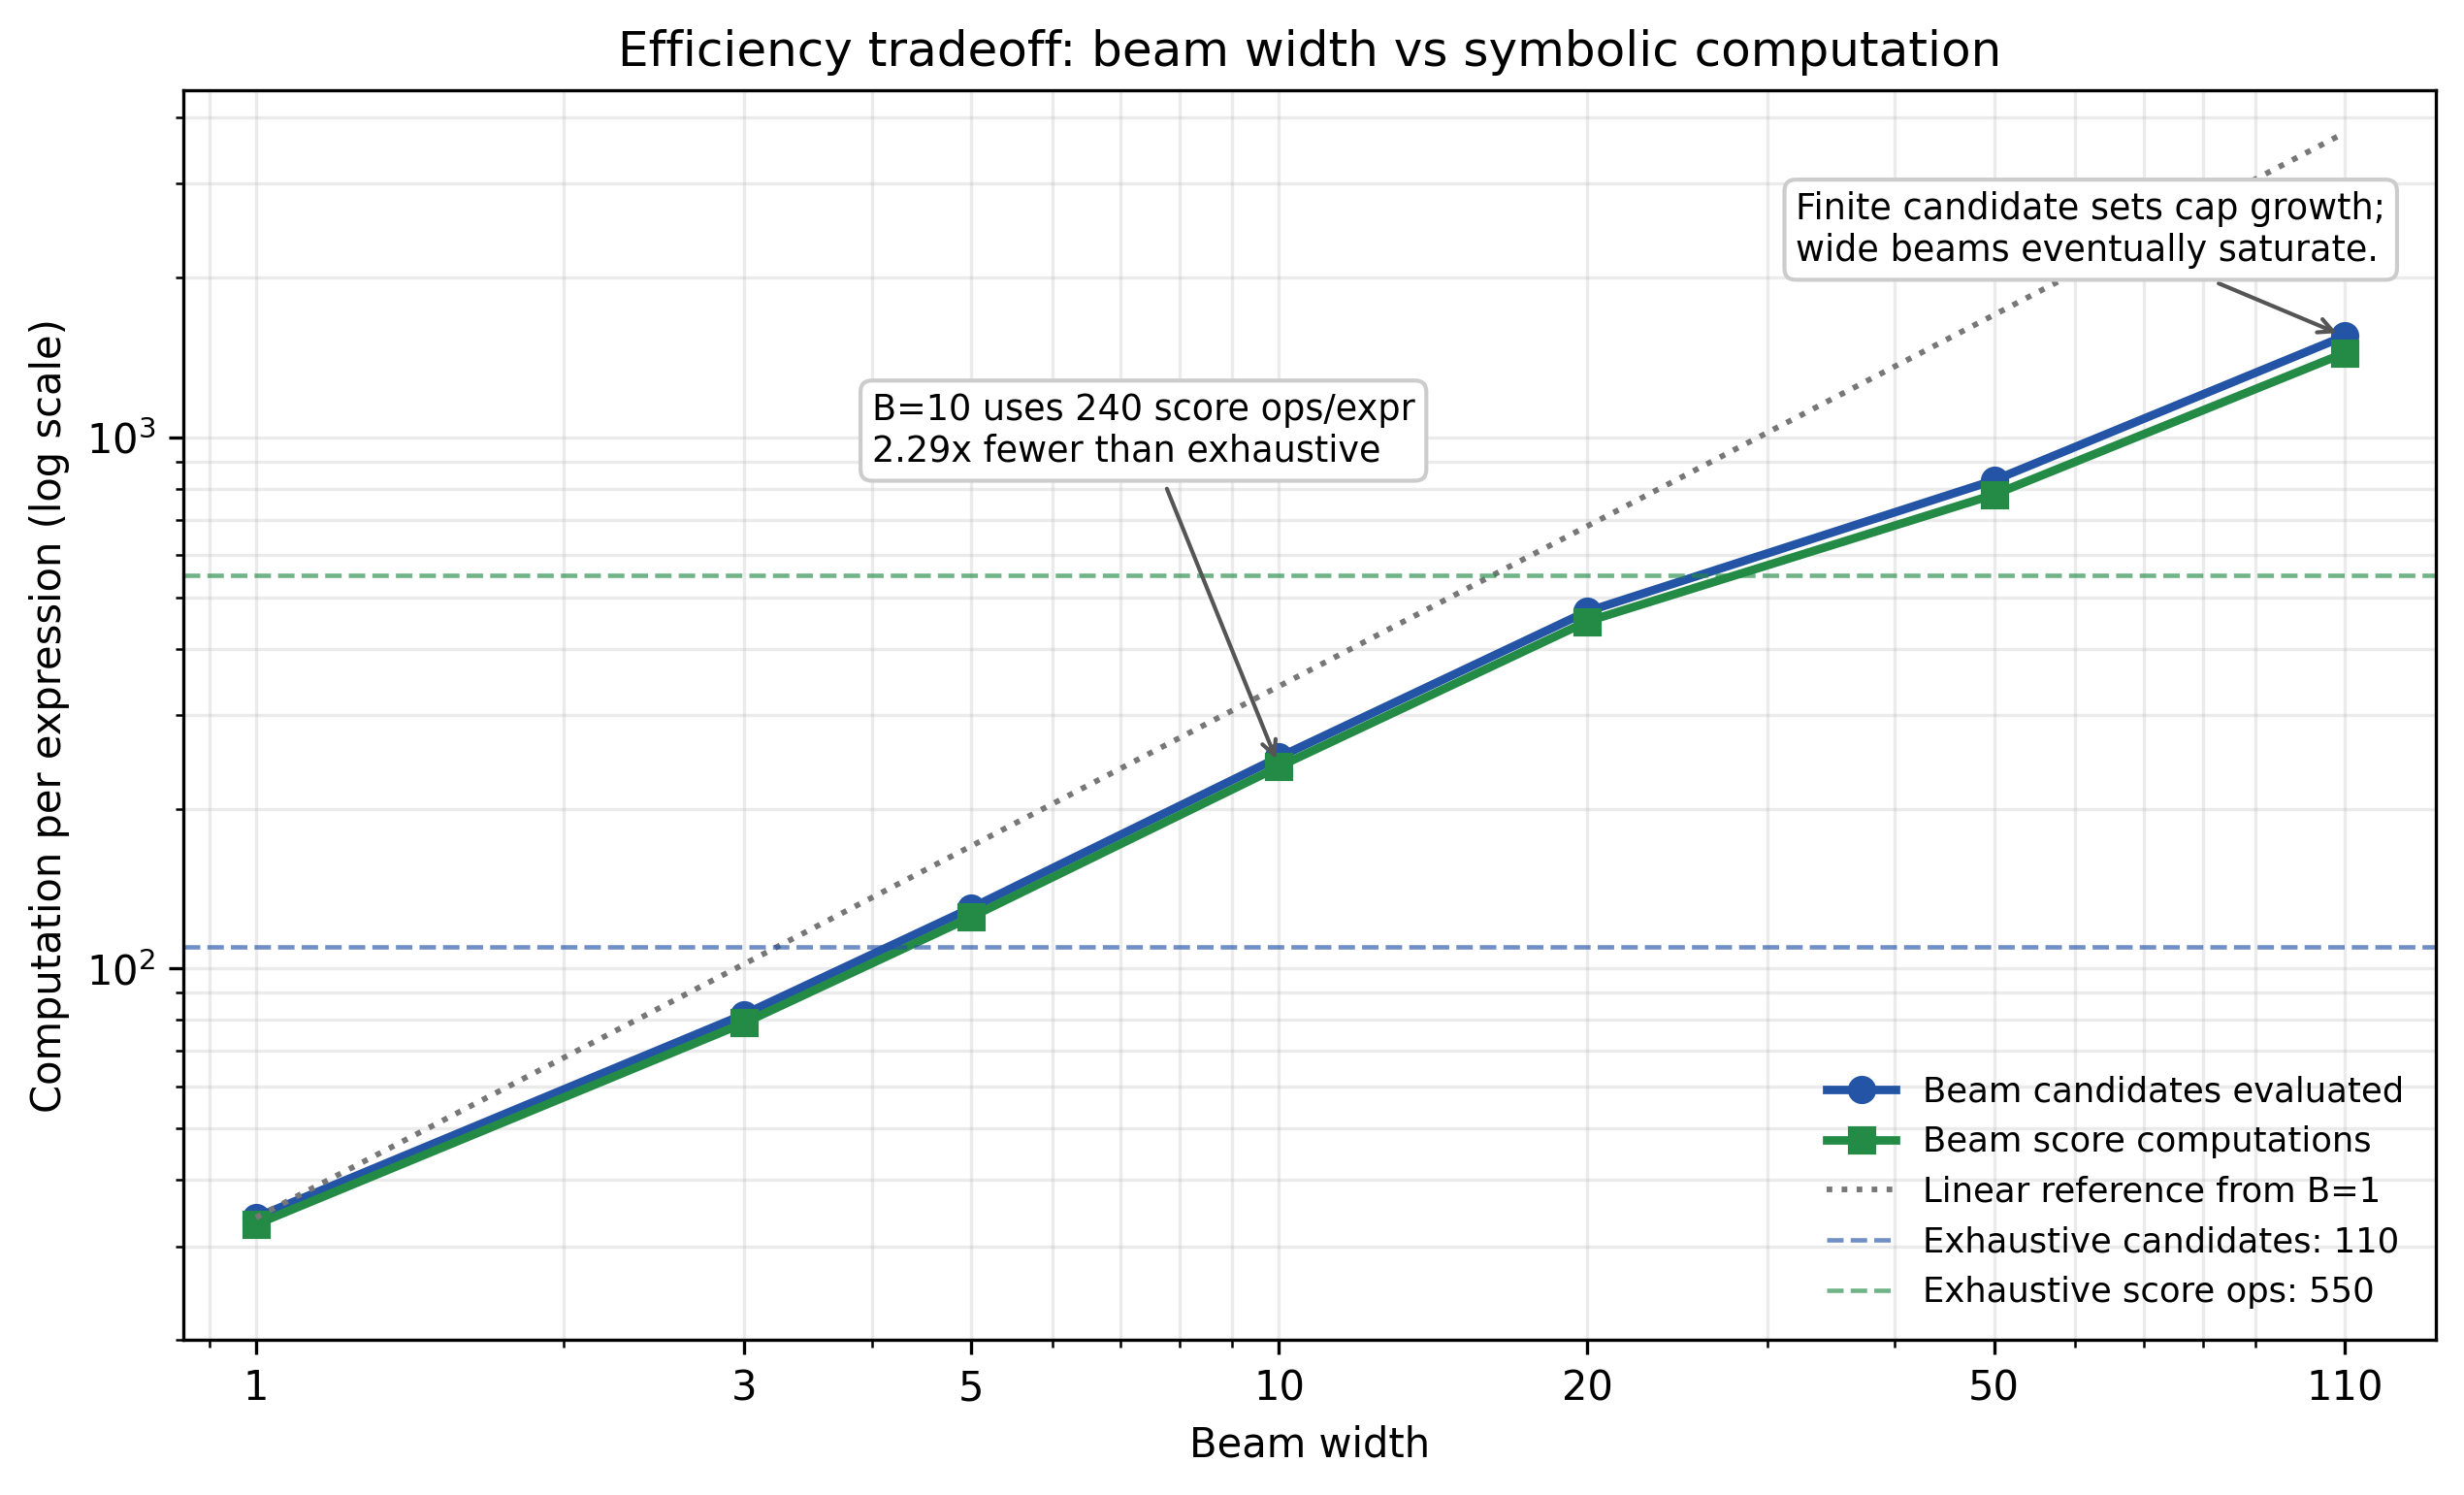
\includegraphics[width=0.78\textwidth]{efficiency_tradeoff.png}
    \caption{Efficiency tradeoff as the beam width increases.}
    \label{fig:efficiency}
\end{figure}

\begin{table}[t]
    \centering
    \caption{Final-beam metrics at $\sigma=0.4$.}
    \label{tab:recoverability}
    \small
    \begin{tabular}{lrrrrr}
        \toprule
        Beam & In beam (\%) & Mean rank & Median & Pruned (\%) & Accuracy (\%) \\
        \midrule
        $B=1$ & 59.96 & 1.00 & 1 & 40.04 & 59.96 \\
        $B=3$ & 83.82 & 1.01 & 1 & 16.18 & 82.62 \\
        $B=5$ & 90.56 & 1.03 & 1 & 9.44 & 88.14 \\
        $B=10$ & 96.18 & 1.04 & 1 & 3.82 & 92.38 \\
        $B=20$ & 98.66 & 1.06 & 1 & 1.34 & 93.66 \\
        $B=50$ & 99.72 & 1.07 & 1 & 0.28 & 93.80 \\
        $B=110$ & 99.96 & 1.08 & 1 & 0.04 & 93.80 \\
        \bottomrule
    \end{tabular}
\end{table}

At $\sigma=0.6$, $B=110$ retains the correct equation in the final beam for 80.26\% of examples, while equation accuracy stands at only 41.98\%. Even when every valid equation is considered by construction, equation accuracy remains at 41.98\%. The failure mode in these cases is not the search process but the scoring function, because the CNN consistently assigns a higher probability to a different valid equation than to the ground-truth equation.

\begin{figure}[t]
    \centering
    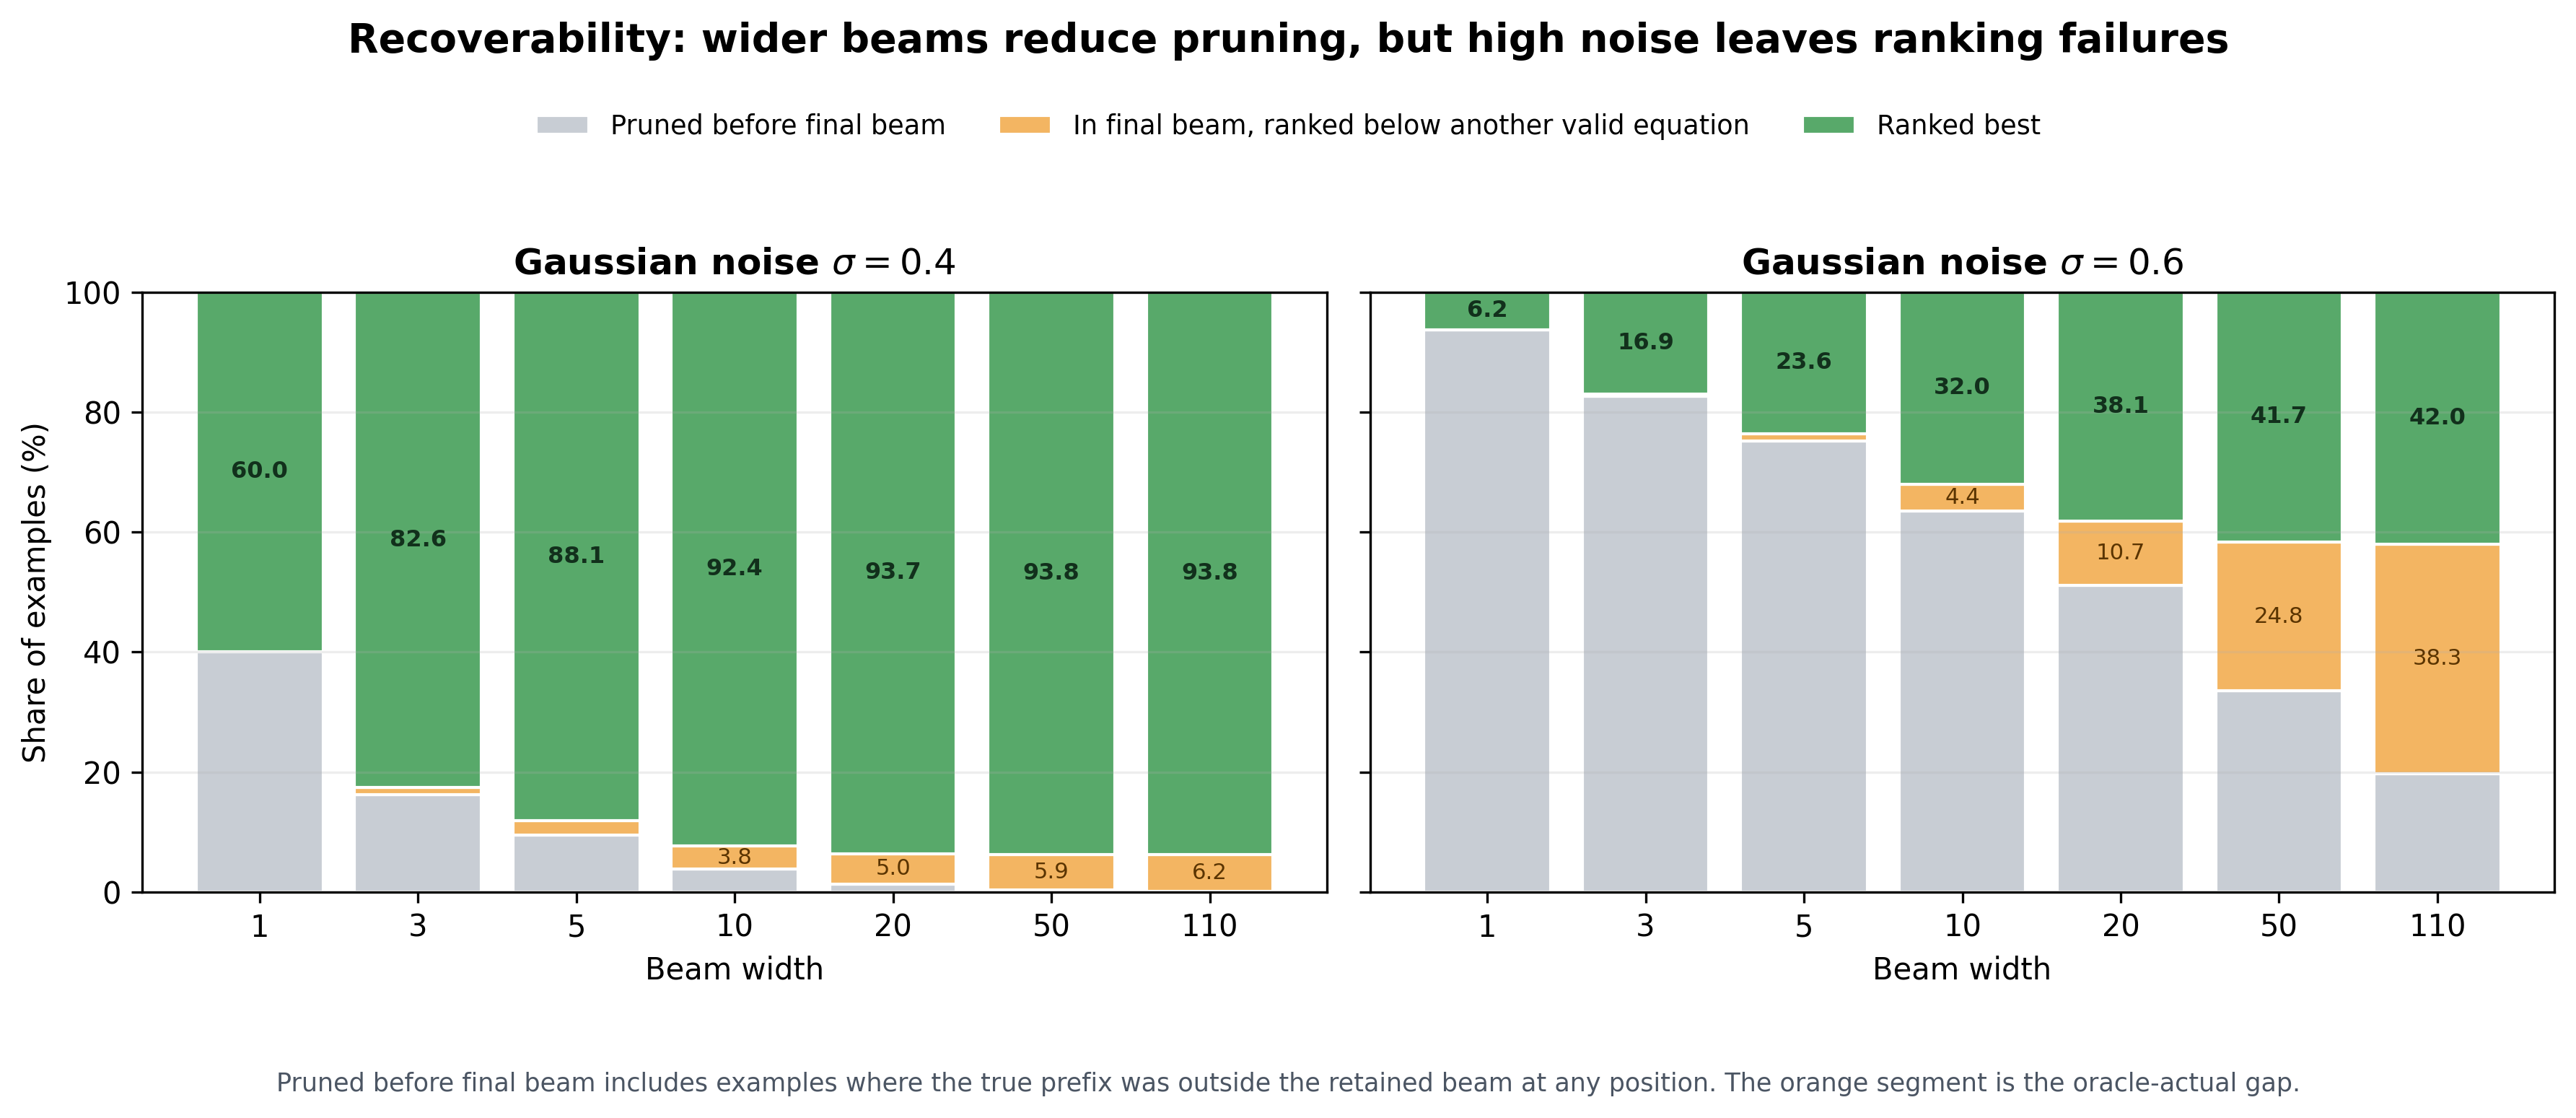
\includegraphics[width=0.9\textwidth]{recoverability_analysis.png}
    \caption{Search-error decomposition under moderate and severe Gaussian noise.}
    \label{fig:recoverability}
\end{figure}

\section{Discussion}
The experiments support two related observations about constrained decoding from neural probabilities. First, requiring arithmetic validity improves equation recognition whenever the CNN still gives the correct symbols reasonably high probabilities. Second, beam width determines whether that probability survives the search procedure long enough to influence the final decision, so that larger beams approach the exhaustive reference by reducing premature pruning of the correct equation.

The arithmetic task used here is simple, but the same kind of decoding problem appears in many other settings. For example, labels extracted from documents may need to follow a required format~\cite{peng2006}. In program synthesis, predicted tokens must form a valid program that actually does what it is supposed to do~\cite{gulwani2017}. In scene understanding, object predictions may need to respect spatial or physical constraints~\cite{mao2019}. These tasks are much larger and harder than five-symbol arithmetic, but they share the same basic need. The system has to keep more than one possible interpretation open until a full output can be checked against a global constraint.

The present experiment does not show that beam search is the best decoder for these larger domains. Its purpose in this paper is different. Because the valid set is small, exhaustive decoding provides a reference point for what exact constrained decoding would choose. Beam search can then be evaluated by comparing its output to that reference. The task includes candidate labels, a neural scoring function, and a validity checker, while beam width controls how many partial structures are kept during decoding.

Several other structured-prediction methods may be better choices in specific situations. A CRF or structured SVM would work better when the model needs to learn sequential patterns from data. A factor graph or integer-programming decoder would make sense when exact optimization is still practical. A probabilistic logic system would be more useful when the system has to combine many uncertain facts, reusable rules, hidden relationships, or multiple possible reasoning paths. In the arithmetic task, however, these benefits matter less because the constraint is deterministic, the layout is fixed, and the valid set is small. A probabilistic logic program would make the system more flexible, but it would not necessarily improve performance on this particular benchmark.

The efficiency result should also be interpreted carefully. In this experiment, $B=10$ is not faster than exhaustive decoding because the reference method only scores 110 equations. The more important point is about how the method scales. Beam search makes computation depend on beam width and sequence length, rather than on the total number of valid complete outputs. This matters when the valid set is too large or changes too often to list ahead of time.

The difference between pruning failures and ranking failures is important for interpreting the method. A narrow beam can fail by removing the correct partial structure before the symbolic constraint can be checked. In those cases, widening the beam can help because the useful evidence is still present in the neural probabilities. A ranking failure is different. The correct complete structure is still available within the beam, but the neural model assigns higher probability to another valid structure. Wider beams cannot fix this type of failure. They only make the problem easier to see. When oracle accuracy is high but actual accuracy is lower, the scoring model is the bottleneck. When oracle accuracy is low and improves as beam width increases, early pruning is the bottleneck.

\section{Limitations}
The benchmark is intentionally simple, so the claims drawn from it should also be limited. The only handwritten symbols in the dataset are MNIST digits, while the plus, minus, and equality signs are rendered glyphs. As a result, the experiment tests uncertainty in digit recognition much more than uncertainty in full mathematical handwriting. Real handwritten equations would also introduce operator variation, inconsistent spacing, touching symbols, stray marks, writer-specific style, and ambiguous layout, all of which could change both the neural error patterns and the effect of the symbolic constraint.

The system also assumes that segmentation and layout are already handled. Each input is split into five known $28 \times 28$ crops, and the decoder is given the fixed template digit, operator, digit, equality sign, digit. It does not detect symbol boundaries, parse two-dimensional notation, infer reading order, or decide whether the input actually has the expected equation format. This makes the task much simpler. As a result, the findings apply to fixed-slot recognition after segmentation, not to unrestricted mathematical expression parsing.

The arithmetic grammar is also narrow. It only allows single-digit addition and subtraction, with no carries, borrows, negative results, parentheses, multi-digit numbers, operator precedence, or variable-length expressions. This simplicity makes the search behavior easier to measure and allows an exact reference decoder. However, it is still much simpler than the larger tasks that motivate structured prediction. In more complex settings, validity may depend on syntax, meaning, types, units, or execution behavior rather than a single arithmetic check.

Beam search also adds an approximation parameter. Unlike the exact reference decoder, beam search requires choosing a beam width $B$, and small beams can remove the correct prefix too early. The best width may depend on the neural model, the noise level, the output length, and the number of possible labels at each step. Because of this, a width that works well for five-symbol equations may not work as well for longer outputs. Wider beams also do not fix ranking errors. When the neural model gives a higher score to an incorrect valid equation, keeping more candidates only makes the failure easier to observe without fixing the scoring problem.

Finally, the comparison with other structured-prediction methods is based on ideas rather than direct experiments. The symbolic module is a constrained beam decoder. It is not a full probabilistic logic program, CRF, factor graph, ILP decoder, or learned neural structured decoder. The Gaussian noise model is mainly used as a controlled way to study how recognition errors affect decoding, not as a complete model of real image degradation. These choices make the experiment easier to reproduce and interpret, but they do not support a general ranking of neuro-symbolic methods.

\section{Future Work}
A natural first step for future work is to remove some of the assumptions that make the current benchmark easy to control. A more realistic dataset would include handwritten plus, minus, equality, and other operator symbols. It would also include variable spacing, segmentation errors, and differences across writers and full expressions. This would allow the system to be tested on perception, slot detection, and constrained decoding together, rather than only on fixed-position symbol classification.

Another technical extension would be to expand the grammar. Multi-digit numbers, carries, borrows, negative results, multiplication, division, parentheses, operator precedence, and variable-length expressions would create a much larger search problem. In these settings, exact decoding would likely become impractical, so beam search would face a stronger test. The main question would be whether it can control a growing set of candidates while still keeping reasonable alternatives available. These settings would also require richer validity checks, such as grammar parsers, expression evaluators, or constraint solvers.

A further direction is to compare the method directly with other structured-prediction approaches. CRFs and structured SVMs could test whether learned local or sequential patterns improve recognition. Factor graphs, ILP decoders, and constraint-programming methods could test exact or optimized inference under explicit constraints. Grammar-based parsers could test whether syntactic structure should guide the search process instead of being checked only at the end. Probabilistic logic systems such as ProbLog or DeepProbLog would be especially useful when rules can be reused, facts are uncertain, and multiple reasoning paths can support the same prediction.

Another line of work concerns training, calibration, and reranking. The CNN used here is trained with local cross-entropy loss, so it is not directly trained to keep globally useful alternatives available. Constraint-aware training and sequence-level losses could be explored with beam-search-aware objectives~\cite{wiseman2016}. Better probability calibration could also make neural scores more reliable for ranking valid candidates~\cite{guo2017}. These changes would matter most in high-noise settings, where the correct equation may still be present in the beam but loses to another valid equation with a higher neural score.

The diagnostic framework could also be extended. The difference between oracle accuracy and actual accuracy is useful because it helps identify the source of failure. Low oracle accuracy points to search pruning or weak local evidence. High oracle accuracy combined with lower actual accuracy points to a scoring failure. Future systems could use this distinction during development to decide whether to widen the beam, improve calibration, add a reranker, or change the constraint representation. Testing the same diagnostic in larger domains would help show how well the findings from the arithmetic task carry over to more complex problems.

\section{Conclusion}
This work presented a controlled neuro-symbolic system for fixed-layout arithmetic expressions made from MNIST digits and rendered operators. A compact CNN produced symbol probabilities for each position, and a beam search decoder used those probabilities to search for equations that satisfied a hard arithmetic constraint. Although the task is small, it highlights that the most likely symbol at each position does not always produce the best complete output. Symbolic validity is useful only when the system keeps enough uncertainty available. Beam search helps because it keeps multiple partial equations open long enough for the arithmetic rule to remove invalid completions. Under moderate noise, increasing the beam width improves both equation accuracy and oracle accuracy, which suggests that many remaining errors depend on the search process. Under severe noise, the constraint can no longer make up for poor neural scores. In those cases, the correct equation may still be in the beam or even considered by the exact reference decoder, but another valid equation receives a higher score.

These results have both a diagnostic message and an algorithmic message. A constrained decoder helps separate pruning failures from ranking failures. When the correct equation disappears from the beam, the beam may be too narrow, or the neural model may give the correct symbols too little support. When the correct equation stays in the beam but is ranked below another valid equation, the scoring model is the bottleneck. This distinction is easy to miss when evaluation reports only final equation accuracy. Beam search does not replace accurate perception, learned structured models, or richer probabilistic logic systems. Instead, it serves as a clear decoding baseline for problems where local neural predictions are uncertain, outputs must satisfy hard constraints, and the correct structured output is still reachable. Beam width gives direct control over how many candidates are kept during decoding, while oracle analysis helps identify whether remaining errors come from search or scoring.

\newpage

\begin{thebibliography}{99}

\bibitem{bakir2007}
G. Bakir, T. Hofmann, B. Sch\"olkopf, A. J. Smola, B. Taskar, and S. V. N. Vishwanathan, editors.
\newblock \textit{Predicting Structured Data}.
\newblock MIT Press, 2007.

\bibitem{lafferty2001}
J. Lafferty, A. McCallum, and F. Pereira.
\newblock Conditional Random Fields: Probabilistic Models for Segmenting and Labeling Sequence Data.
\newblock In \textit{Proceedings of the 18th International Conference on Machine Learning}, pages 282--289, 2001.

\bibitem{tsochantaridis2005}
I. Tsochantaridis, T. Joachims, T. Hofmann, and Y. Altun.
\newblock Large Margin Methods for Structured and Interdependent Output Variables.
\newblock \textit{Journal of Machine Learning Research}, 6:1453--1484, 2005.

\bibitem{collins2004}
M. Collins and B. Roark.
\newblock Incremental Parsing with the Perceptron Algorithm.
\newblock In \textit{Proceedings of the 42nd Annual Meeting of the Association for Computational Linguistics}, pages 111--118, 2004.

\bibitem{peng2006}
F. Peng and A. McCallum.
\newblock Information Extraction from Research Papers Using Conditional Random Fields.
\newblock \textit{Information Processing \& Management}, 42(4):963--979, 2006.

\bibitem{gulwani2017}
S. Gulwani, O. Polozov, and R. Singh.
\newblock Program Synthesis.
\newblock \textit{Foundations and Trends in Programming Languages}, 4(1--2):1--119, 2017.

\bibitem{mao2019}
J. Mao, C. Gan, P. Kohli, J. B. Tenenbaum, and J. Wu.
\newblock The Neuro-Symbolic Concept Learner: Interpreting Scenes, Words, and Sentences From Natural Supervision.
\newblock In \textit{International Conference on Learning Representations}, 2019.

\bibitem{zanibbi2012}
R. Zanibbi and D. Blostein.
\newblock Recognition and Retrieval of Mathematical Expressions.
\newblock \textit{International Journal on Document Analysis and Recognition}, 15(4):331--357, 2012.

\bibitem{sutskever2014}
I. Sutskever, O. Vinyals, and Q. V. Le.
\newblock Sequence to Sequence Learning with Neural Networks.
\newblock In \textit{Advances in Neural Information Processing Systems 27}, 2014.

\bibitem{bahdanau2015}
D. Bahdanau, K. Cho, and Y. Bengio.
\newblock Neural Machine Translation by Jointly Learning to Align and Translate.
\newblock In \textit{International Conference on Learning Representations}, 2015.

\bibitem{hendrycks2019}
D. Hendrycks and T. Dietterich.
\newblock Benchmarking Neural Network Robustness to Common Corruptions and Perturbations.
\newblock In \textit{International Conference on Learning Representations}, 2019.

\bibitem{lecun1998}
Y. LeCun, L. Bottou, Y. Bengio, and P. Haffner.
\newblock Gradient-Based Learning Applied to Document Recognition.
\newblock \textit{Proceedings of the IEEE}, 86(11):2278--2324, 1998.

\bibitem{kingma2015}
D. P. Kingma and J. Ba.
\newblock Adam: A Method for Stochastic Optimization.
\newblock In \textit{International Conference on Learning Representations}, 2015.

\bibitem{manhaeve2018}
R. Manhaeve, S. Dumancic, A. Kimmig, T. Demeester, and L. De Raedt.
\newblock DeepProbLog: Neural Probabilistic Logic Programming.
\newblock In \textit{Advances in Neural Information Processing Systems 31}, pages 3753--3763, 2018.

\bibitem{deraedt2007}
L. De Raedt, A. Kimmig, and H. Toivonen.
\newblock ProbLog: A Probabilistic Prolog and Its Application in Link Discovery.
\newblock In \textit{Proceedings of the 20th International Joint Conference on Artificial Intelligence}, pages 2468--2473, 2007.

\bibitem{dong2019}
H. Dong, J. Mao, T. Lin, C. Wang, L. Li, and D. Zhou.
\newblock Neural Logic Machines.
\newblock In \textit{International Conference on Learning Representations}, 2019.

\bibitem{kschischang2001}
F. R. Kschischang, B. J. Frey, and H.-A. Loeliger.
\newblock Factor Graphs and the Sum-Product Algorithm.
\newblock \textit{IEEE Transactions on Information Theory}, 47(2):498--519, 2001.

\bibitem{roth2004}
D. Roth and W.-T. Yih.
\newblock A Linear Programming Formulation for Global Inference in Natural Language Tasks.
\newblock In \textit{Proceedings of the Eighth Conference on Computational Natural Language Learning}, pages 1--8, 2004.

\bibitem{wiseman2016}
S. Wiseman and A. M. Rush.
\newblock Sequence-to-Sequence Learning as Beam-Search Optimization.
\newblock In \textit{Proceedings of the 2016 Conference on Empirical Methods in Natural Language Processing}, pages 1296--1306, 2016.

\bibitem{guo2017}
C. Guo, G. Pleiss, Y. Sun, and K. Q. Weinberger.
\newblock On Calibration of Modern Neural Networks.
\newblock In \textit{Proceedings of the 34th International Conference on Machine Learning}, pages 1321--1330, 2017.

\end{thebibliography}

\appendix
\section{Algorithms}
\label{app:algorithms}

\begin{algorithmbox}{alg:beam-search}{Beam Search Decoder}
\algmeta{Input}{Per-position probabilities $p_i(k)$, beam width $B$, candidate-label function $C(i)$, validity function $Valid(\mathbf{y})$.}
\algmeta{Output}{Highest-scoring valid assignment, or no prediction if the final beam contains no valid assignment.}
\algstep{1}{Set $beam \leftarrow \{(\langle\rangle, 0)\}$.}
\algstep{2}{\textbf{for} each position $i = 1,\dots,5$ \textbf{do}}
\algstep{3}{\hspace*{1em}Set $expanded \leftarrow \emptyset$.}
\algstep{4}{\hspace*{1em}\textbf{for} each $(\mathbf{y}, s) \in beam$ and each label $k \in C(i)$ \textbf{do}}
\algstep{5}{\hspace*{2em}Add $(\mathbf{y} \circ k,\; s + \log p_i(k))$ to $expanded$.}
\algstep{6}{\hspace*{1em}\textbf{end for}}
\algstep{7}{\hspace*{1em}Set $beam$ to the top $B$ assignments in $expanded$ by score.}
\algstep{8}{\textbf{end for}}
\algstep{9}{Set $valid \leftarrow \{(\mathbf{y}, s) \in beam : Valid(\mathbf{y})\}$.}
\algstep{10}{\textbf{if} $valid = \emptyset$ \textbf{then} return no prediction.}
\algstep{11}{\textbf{else} return the assignment in $valid$ with maximum score.}
\end{algorithmbox}

\begin{algorithmbox}{alg:valid-equation}{Arithmetic Validity Check}
\algmeta{Input}{A complete five-symbol assignment $\mathbf{y} = (y_1,y_2,y_3,y_4,y_5)$.}
\algmeta{Output}{Boolean value indicating whether $\mathbf{y}$ is a valid equation.}
\algstep{1}{\textbf{if} $y_1,y_3,y_5$ are not digits, return false.}
\algstep{2}{\textbf{if} $y_2 \notin \{+,-\}$ or $y_4 \neq \text{=}$, return false.}
\algstep{3}{\textbf{if} $y_2 = +$, return whether $y_1 + y_3 = y_5$.}
\algstep{4}{\textbf{if} $y_2 = -$, return whether $y_1 - y_3 = y_5$.}
\end{algorithmbox}

\end{document}
